\subsection{Non-Classical Logic}
\subsubsection{Non-Classical Propositional Logic}

If an object $x$ stands in the relation $R$ to object $y$, we write $R(x,y)$, otherwise $\sim R(x,y)$\\

Def: $R$ is reflexive iff for all $x$, $R(x,x)$\\
eg. $R(x,y)$ is ``$x$ is the father of $y$" is not reflexive\\
$R(x,y)$ is ``$x$ is identical to $y$" is reflexive\\

Def: $R$ is symmetric iff for all pairs of objects $x,y$ if $R(x,y)$ then $R(x,y)$\\
eg. $R$ is ``$x$ is the father of $y$" is not symmetric\\
$R$ is ``$x$ is identical to $y$" is symmetric\\

Def: $R$ is transitive iff for all triangles of objects $x,y,z$ if $R(x,y)\& R(y,z)$ then $R(x,z)$\\
eg. $R$ is ``$x$ is the father of $y$" is not transitive\\
$R$ is ``$x$ is to the left of $y$" is transitive

Def: $R$ is equivalence iff $R$ is reflexive, symmetric, and transitive.\\

Def: $R$ is a partial order iff $R$ is reflexive, transitive, and antisymmetric\\

System RP:\\
Relation $R$ is written $R(p,q)$ and is read ``$p$ is related to $q$".\\
It holds between propositions that share a common subject matter

Ex: $A$=``Plato was a student of Socrates"\\
$B$=``Aristotle was a student of Plato"\\
$C$=``Aristotle was a great logician"\\
Topics mentioned in A: \{Plato, student, Socrates\}\\
Topics mentioned in B: \{Aristotle, student, Plato\}\\
Topics mentioned in C: \{Aristotle, logician\}\\
$R(A,B)$ is true and $R(B,A)$ is true\\
$R(B,C)$ is true and $R(C,B)$ is true\\
Also $\sim R(A,C)$ and $\sim R(C,A)$\\
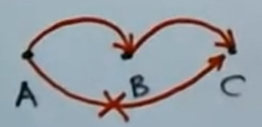
\includegraphics[scale=1]{Images/Phil120Pictures/image1.png}\\
So the system in not transitive\\

\begin{tabular}{ccccc}
    $p$ & $q$ & $R(p,q)$ & $p\to q$ & $p\leftrightarrow q$\\
    \hline
    T & T & T & T & T\\
    T & F & T & F & F\\
    F & T & T & T & F\\
    F & F & T & T & T\\
    T & T & F & F & F\\
    T & F & F & F & F\\
    F & T & F & F & F\\
    F & F & F & F & F
\end{tabular}\\
\begin{tabular}{ccc}
    $p$ & $R(p,p)$ & $\lnot p$\\
    \hline
    T & T & F\\
    F & T & T
\end{tabular}\\
\begin{tabular}{ccccc}
    $p$ & $q$ & $R(p,q)$ & $p\wedge q$ & $p\vee q$\\
    \hline
    T & T & T & T & T\\
    T & F & T & F & T\\
    F & T & T & F & T\\
    F & F & T & F & F\\
    T & T & F & T & F\\
    T & F & F & F & F\\
    F & T & F & F & F\\
    F & F & F & F & F
\end{tabular}\\
Ex: $A$=``Plato was a student of Socrates"\\
$B$=``Aristotle was a student of Plato"\\
$C$=``Aristotle was a great logician"\\
Is $\lnot B\to(A\vee \lnot C)$ true or false?\\
$R(A,B)$, $R(B,C)$, $\sim R(A,C)$\\
Topics in $\lnot C$ are the same as topics in $C$ so we have $\sim R(A,\lnot C)$\\
So $A\vee \lnot C$ is F\\
Topics in $A\vee \lnot C$: topics in $A$ + topics in $\lnot C$ = \{Plato, students, Socrates, Aristotle, logician\}\\
$R(\lnot B,(A\vee\lnot C))$ is true\\
We have $\lnot B$ is F and $A\vee\lnot C$ is F so $\lnot B\to(A\vee\lnot C)$ is T\\

Ex2: Is the formula $(p\to q)\to(\lnot p\vee q)$ a tautology, contingency, or contradiction?\\
This would be done with a truth table\\

Ex3:\\
\argument{4}{$A\to C$\\
$B\to D$\\
$\lnot C\vee\lnot D$\\
\hline
$\therefore \lnot A\vee \lnot B$
}\\
$A\to C$ is T so $R(A,C)$ is T\\
$B\to D$ is T so $R(B,D)$ is T\\
$\lnot C\vee \lnot D$ is T so $R(C,D)$ is T\\
but $R(A,B)$ is F so $\lnot A\vee\lnot B$ is F\\

Aristotle's problem of future contingents:\\
Ex: ``Athens will win the sea battle tomorrow"\\
We can analyze cases like this using Lucasiewicz's Logic\\
This introduces a third truth value, I, meaning indeterminate/unknown\\
Analyzing these cases,\\
\begin{tabular}{cc|cccc}
    $p$ & $q$ & $p\& q$ & $p\vee q$ & $p\supset q$ & $p\equiv q$\\
    \hline
    T & I & I & T & I & I\\
    F & I & F & I & T & I\\
    I & T & I & T & T & I\\
    I & F & F & I & I & I\\
    I & I & I & I & T & T
\end{tabular}\\

Bochvor's System:\\
This deals with paradoxical systems and any operation involving and I will result in I.

\subsubsection{Term Logic}

Subject + Predicate\\
Ex: Victoria is the capital of BC\\
Victoria is the subject and ``is the capital of BC" is the predicate\\
This refers to a single individual object\\
Called \textit{singular sentence}\\

Ex2: Dogs are nice (creatures)\\
refers to a class/group/category//
called \textit{categorical sentence}\\
Def: A categorical sentence is one in which both subject and predicate are classes/sets/categories of objects that states an inclusion (or exclusion) relation between these two classes.\\

Term logic:\\
Capital letters stand for a description of a set/group of objects (with some property)\\
Ex: P=``UBC students", Q=``Dogs that like to chase cats", R=``Nice creatures"\\

Ex: All dogs are mammals\\
dogs are the subject and ``are" is called the \textit{copula}. Mammals is the predicate class.\\
This is \textit{total inclusion} (dogs is a subset of mammals)
Ex2: No dogs are cats\\
This is \textit{total exclusion} (the two sets have no overlap)\\
Ex3: Some dogs are US presidents\\
dogs is the subject, US presidents is the predicate class.\\
Some is defined as ``There exists at least one"\\
This is \textit{partial inclusion} (at least one object belongs to both sets)\\
Ex4: Some dogs are not UBC students\\
This is \textit{partial exclusion} (at least one object does not belong to both sets)\\

Types of claims:
\begin{itemize}
\item A: All $S$ are $P$ (universal affirmative)\\
If you're in $S$ then you're in $P$. ($p\supset q)$
\item E: No $S$ are $P$ (universal negative)\\
If you're in $S$ then you're not in $P$ ($p\supset\sim q$)
\item I: Some $S$ are $P$ (particular affirmative)\\
There exists at least one $S$ which is also in $P$
\item O: Some $S$ are not $P$ (particular negative)
\end{itemize}
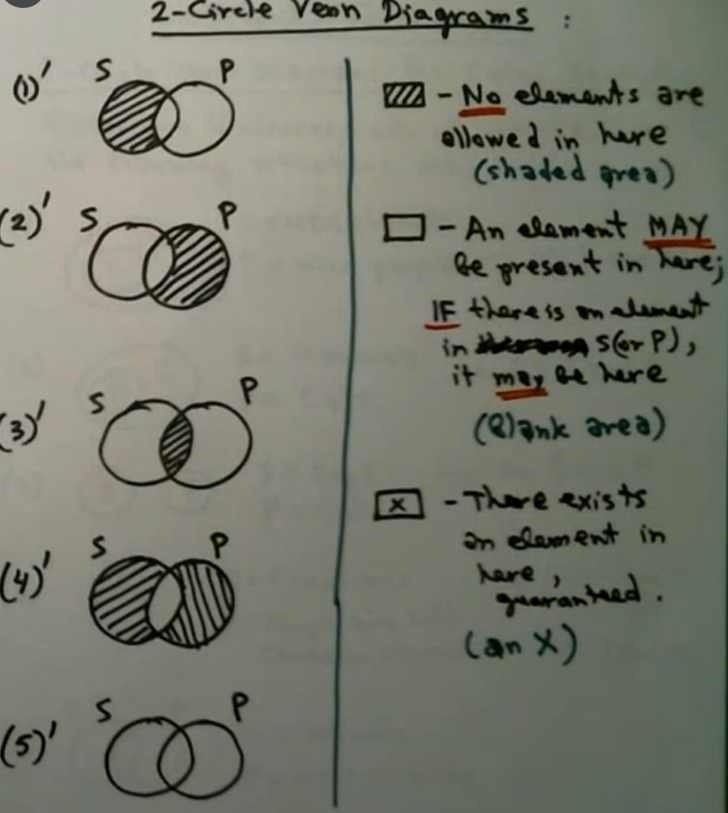
\includegraphics[scale=0.8]{Images/Phil120Pictures/image2.png}\\

Def: The \textit{converse} of a categorical proposition is obtained by interchanging the proposition's subject and predicate terms\\
E and I types have their converse equal to their original claims but this is not the case for A and O claims.\\

Immediate inference:\\
Ex:\\
\argument{6}{No senators are politicians\\
\hline
No politicians are senators} (valid, E-conversion)\\
\argument{6}{Some books are valuable objects\\
\hline Some valuable objects are books} (valid, I-conversion)\\
\argument{6}{All students are hard workers\\
\hline
All hard workers are students} (invalid, A-conversion)\\
\argument{6}{Some mammals are not dogs\\
\hline
Some dogs are not mammals} (invalid, O-conversion)\\

The \textit{contrapositive} of a categorical proposition is obtained by converting it and negating both of its two non-logical terms\\
A and O types have their contrapositives equal to their original claims but E and I claims do not.\\

Ex:\\
\argument{7}{All men are mortal creatures\\
\hline All non-mortal creatures are non-men} (valid, A-contraposition)\\
\argument{7}{Some people are not bankers\\
\hline Some non-bankers are not non-people} (valid, O-contraposition)\\
\argument{7}{No students are employees\\
\hline No non-employees are non-students} (invalid, E-contrapostion)\\
\argument{7}{Some objects are red things\\
\hline Some non-red things are non-objects} (invalid, I-contraposition)\\

The \textit{obverse} of a categorical proposition is obtained by negating the predicate term and changing the proposition from affirmative to negative or from negative to affirmative.\\
i.e. All $S$ are $P$ $\to$ No $S$ are non-$P$\\
Some $S$ are $P$ $\to$ Some $S$ are not non-$P$\\
All A,E,I,O propositions are logically equivalent to their obverses\\

Contradiction\\
Given two contradictory propositions, at most one can be true and at most one can be false\\

Contrariety\\
Given two contrary propositions, at most one can be true, although both may be false\\

Subcontrariety\\
Given two subcontrary propositions, at most once can be false although both may be true\\

Ex: Contradiction\\
All human differences are determined by the environment\\
Not all human differences are determined by the environment\\

Ex: Contrariety\\
All human differences are determined by the environment\\
No human differences are determined by the environment\\

Ex: Subcontrariety\\
Some human differences are determined by the environment\\
Some human differences are not determined by the environment\\

Square of opposition:\\
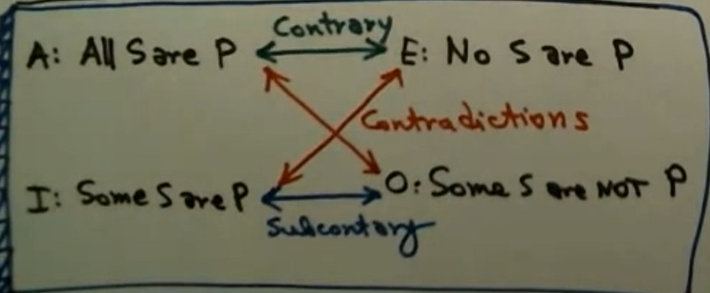
\includegraphics[scale=0.8]{Images/Phil120Pictures/image3.png}\\
Ex: Not all people are cats\\
Not (all $S$ are $P$)\\
= Some $S$ are not $P$\\
Ex2: It's false that no people are students\\
Not (no $S$ are $P$)\\
= Some $S$ are $P$\\
Ex3: It's not true that all cats are not dogs\\
Not (no $S$ are $P$)\\
= Some $S$ are $P$\\

Syllogisms:\\
Def: A \textit{syllogism} is an argument in which there are exactly 3 non-logical referring terms, there are exactly 3 categorical propositions, and each term appears in exactly 2 of these propositions.\\
Ex:\\
\argument{6}{All whales are mammals\\
All mammals are nice\\
\hline All whales are nice}\\
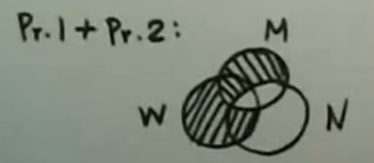
\includegraphics[scale=0.7]{Images/Phil120Pictures/image4.png}\\

Ex2:\\
\argument{5}{All P are L\\Some G are P\\\hline Some G are L}\\
Def: the \textit{major term} appears in the predicate of the conclusion\\
The \textit{minor term} appears in the subject of the conclusion\\
The \textit{middle term} appears in both of the premises but not in the conclusion\\

Def: A referring term is \textit{distributed} iff that proposition says something about every member of that's term extension\\
A: All UBC students are people\\
So students would be distributed\\

In all universal claims (A,E) the subject is distributed\\
In all negative claims (E,O) the predicate is distributed\\

5 Rules for Validity of Syllogisms\\
All syllogisms must have the following:
\begin{itemize}
    \item A middle term that is distributed at least once
    \item Major and minor terms that are distributed in their premises if they are distributed in the conclusion
    \item At least one affirmative premise
    \item A negative conclusion iff one of the premises is negative\\
    i.e a) A negative conclusion and exactly one negative premise or\\
    b) An affirmative conclusion and either 2 premises are negative or none of the premises are negative\\
    The total number of negations must not be odd
    \item A particular premise if the conclusion is particular
\end{itemize}